\documentclass[12pt]{article}
\usepackage{geometry}                % See geometry.pdf to learn the layout options. There are lots.
\geometry{letterpaper}                   % ... or a4paper or a5paper or ... 
%\geometry{landscape}                % Activate for for rotated page geometry
\usepackage[parfill]{parskip}    % Activate to begin paragraphs with an empty line rather than an indent
\usepackage{daves,fancyhdr,natbib,graphicx,dcolumn,amsmath,lastpage,url}
\usepackage{amsmath,amssymb,epstopdf,longtable}
\usepackage{paralist}  % need to properly formulate standard answer blocks
\usepackage[final]{pdfpages}
\DeclareGraphicsRule{.tif}{png}{.png}{`convert #1 `dirname #1`/`basename #1 .tif`.png}
\pagestyle{fancy}
\lhead{CE 3305 Fluid Mechanics; Exercise Set 9}
\rhead{Name:\_\_\_\_\_\_\_\_\_\_\_\_\_\_\_\_\_\_\_\_\_\_\_\_\_\_\_\_\_\_\_\_\_\_}
\lfoot{REVISION A}
\cfoot{}
\rfoot{Page \thepage\ of \pageref{LastPage}}
\renewcommand\headrulewidth{0pt}
%%%%%%%%%%%%%%%%%%%%%%%%%%%%%%%%%%%%
\begin{document}
%%%%%%%%%%%%%%%%%%%%%%%%%%%%%%%%%%%
\begingroup
\begin{center}
{\textbf{{ CE 3305 Engineering Fluid Mechanics} \\ Exercise Set 9 \\ Summer 2018 -- GERMANY} }
\end{center}
\endgroup
\begingroup
~\newline
\textbf{Purpose} :  Static and dynamic pressure.  Bernoulli's equation. \\
\textbf{Assessment Criteria} : Completion, plausible solutions, use \textbf{R} as a calculator. \\~\\
\textbf{Exercises}

\begin{enumerate}
\item (Problem 4.55 pg 161)  Figure \ref{fig:PitotTube} is a schematic of a glass tube inserted into a flowing stream of water with one opening directed upstream and the other end vertical.  If the water velocity is 4 $m/s$, how high will the water rise in the vertical leg relative to the level of the water surface of the stream?

\begin{figure}[htbp] %  figure placement: here, top, bottom, or page
   \centering
   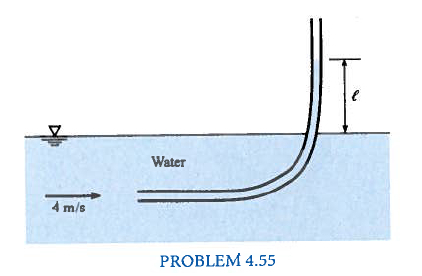
\includegraphics[width=3in]{PitotTube.jpg} 
   \caption{Tube for measuring velocity head.}
   \label{fig:PitotTube}
\end{figure}
\clearpage
(Problem 4.55 pg 161) (Continued)
\clearpage
\item (Problem 4.87 pg 164)  Figure \ref{fig:TankDrain} is a schematic of a reservoir draining into a pipe.   The velocity in the outlet pipe is 8 $m/s$ and $h$=19$m$.  Because of the rounded entrance to the pipe, the flow is assumed to be irrotational.  What is the pressure at $A$?
\begin{figure}[htbp] %  figure placement: here, top, bottom, or page
   \centering
   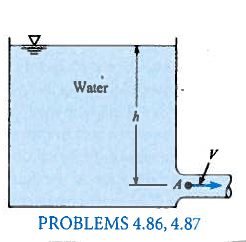
\includegraphics[width=2.5in]{TankDrain.jpg} 
   \caption{Reservoir draining into a penstock (pipe).}
   \label{fig:TankDrain}
\end{figure}
\clearpage
(Problem 4.87 pg 164) (Continued)
\clearpage
\item (Problem 4.91 pg 165).  Figure \ref{fig:AirFoil} is a schematic of ideal flow around an air foil.  If the approach air velocity is $V_0$=80$m/s$, what is the pressure difference between the bottom and the top of this airfoil at points where the velocities are $V_1$=85$m/s$ and $V_2$=75$m/s$?  Assume $\rho_{air}$ is uniform at 1.2~$kg/m^3$.
\begin{figure}[htbp] %  figure placement: here, top, bottom, or page
   \centering
   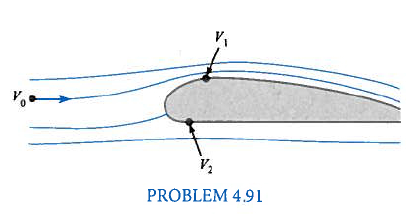
\includegraphics[width=3in]{AirFoil.jpg} 
   \caption{Ideal flow around an airfoil.}
   \label{fig:AirFoil}
\end{figure}
\clearpage
(Problem 4.91 pg 165) (Continued)
\end{enumerate}


\end{document}  